\chapter{関連研究}
%ドライブレコーダーを用いた関連研究について
\section{ドライブレコーダーを用いた研究}
自動車にカメラ及びドライブレコーダーを取り付けて行なった研究として,まず道路のひび割れや塗装の剥がれといったものを検出する研究\cite{全邦釘2017ディープラーニングおよび}がある.
画像処理技術が向上したことで,道路における障害物やひび割れといったものの検出が可能となった.
しかし,道路のひび割れのような不動で固定的なものとは異なり,渋滞というものは時間と共に発生したり解消したり,また規模も大きくなったり小さくなったりと変化するものあり,変化するものに対しての画像認識の対応は困難なものだった.

ドライブレコーダーと機械学習を組み合わせたものとしては,Japan Taxi株式会社が既にタクシーに高性能なドライブレコーダーをつけて,走行中の道路の状況等をリアルタイムに収集し解析するというサービスを行なっている.
しかし,そこで行われているのは歩行者の検出や道路工事の検出などであり,発展して渋滞を推定すると言う旨の実現には至っていない.
各タクシーから集められた情報をもとに人間の手で渋滞かどうか判断しているので,本研究によってその人間の判断を自動化する,あるいは事前に渋滞かどうか疑わしい現場の映像に判断材料を絞ることができる点で,本研究には貢献できる点があると言える.

%車載カメラからの画像処理について書きたい
\section{ドライブレコーダー以外の車載カメラを用いた研究について}
ドライブレコーダー以外の車載カメラの研究について,三上ら\cite{三上量弘2020deepcounter}は,ゴミ収集車にカメラ取り付けるとこで,ゴミ収集車にどれほどのゴミ袋が収集されたかを調べる研究を行った.
ゴミ清掃車は,日々決まったルートを通り,決まった場所でゴミを収集している.
その収集されるゴミの量を数値として可視化することで住民の生活の変化を可視化する研究である.
自動車にカメラを取り付けて,映像情報からデーターを可視化するという目的の点で,可視化するデーターが異なるとはいえ,三上らの研究はこの研究と共通点がある.
また,三上らの研究には私の研究と同様のYOLOと呼ばれる物体検出システムが使用されており,その物体検出システムが検出したゴミ袋の量を計測していた.

以上を踏まえると,物体検出システムを使用することでデーターの可視化が可能であると言える.

\newpage

\section{渋滞推定の研究について}
ドライブレコーダー以外の方法でカメラから渋滞を測定する方法として,進藤ら\cite{進藤瞭2013車載カメラ画像を用いた対向車線の渋滞状況の把握手法}は,対向車の交通量を測定することで渋滞を推定する研究を行なった.
進藤らの方法は自動車2台を走行させ,その2台の横を通過した対向車の数から渋滞しているか否かを判断するものである.
しかし,進藤らの方法では測定するための自動車は常に道路の右側車線を走行しなければならないと同時に,対向車道がない道路では渋滞を推定することができないという問題がある.

\section{カメラを用いた距離推定の研究}
%センサー情報を含めた先行研究
車間距離を推定するフェーズに関して,動画から距離を推定する方法はいくつか存在する.
まず最も簡単かつ確実な方法は複眼カメラと三角関数を利用した方法である.
同じ対象を移したときに2つの視点からそれぞれのカメラから対象の距離を測定する方法である.
しかし,本研究の対象はドライブレコーダーであり,1つの自動車に2つのドライブレコーダーを搭載することは現実的ではなく,複眼のドライブレコーダーは一般的に搭載されていないためこの方法は利用できない.
そのため,この研究では単眼カメラの映像から車間距離を推定する必要がる.
単眼カメラから物体との距離を推定する研究としては,カメラ情報に加えて各種距離センサーの情報を利用することで実現する方法が一般的であった.

% Struct2depth
しかし,近年ではDeep Learning技術の向上により,各種センサーといった教師データーのない,純粋に画像のみでの距離推定プログラムが実現している.
Zhouら\cite{zhou2017unsupervised}はセンサー情報等の教師データのないカメラ映像から奥行きを推定するシステムを開発した.
Zhouらのシステムは,車載動画等の連続的な画像の集まりであるデータセットを元に映像における視界の変化を元に奥行きを推定するものであった.
Zhouらの研究以降,カメラ映像における奥行きの研究は,Zhouらの研究を元に性能向上がなされ,Yinら\cite{yin2018geonet}などによってアップデートがなされた.

中でも,Googleの研究チームのCasserらが行なった研究である"Struct2Depth"\cite{casser2019struct2depth}というシステムは上記の研究と比較して精度がより向上されている\figref{fig:depth_related}.
本研究ではStruct2Depthを利用し,車間距離を推定する.

\newpage

\begin{figure}[hp]
  \begin{center}
   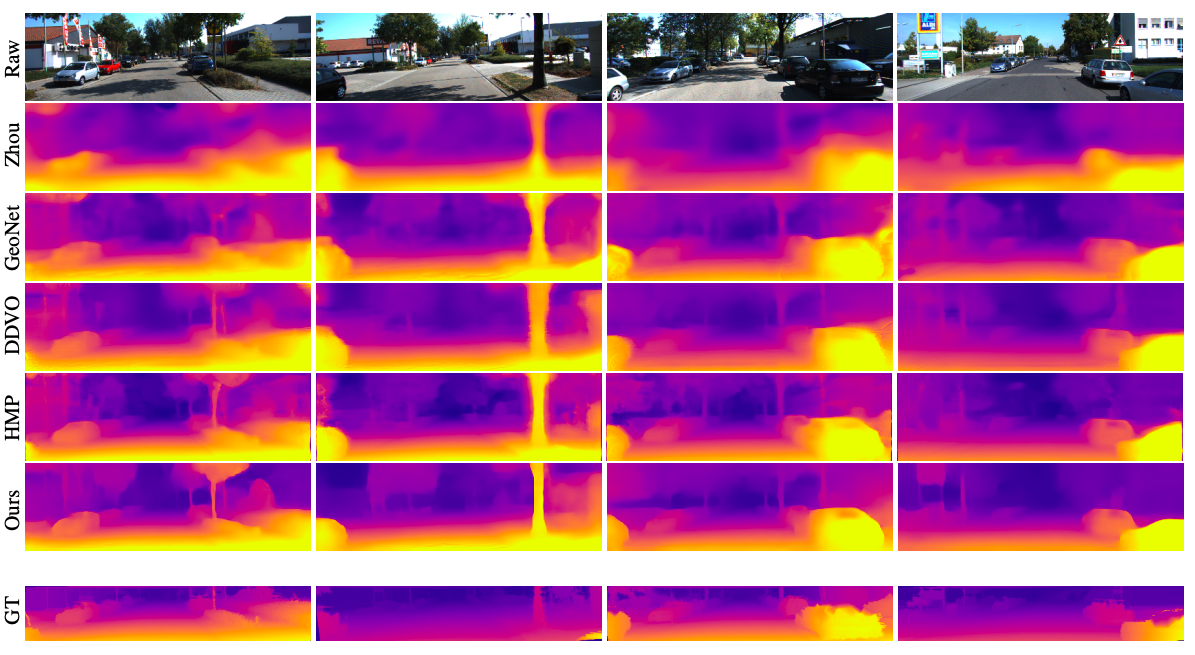
\includegraphics[width=\textwidth]{figs/struct2depth_related.png}
  \end{center}
  \caption{struct2depthと他の研究の比較\cite{casser2019struct2depth}}
  \label{fig:depth_related}
\end{figure}

\begin{figure}[hp]
  \begin{center}
   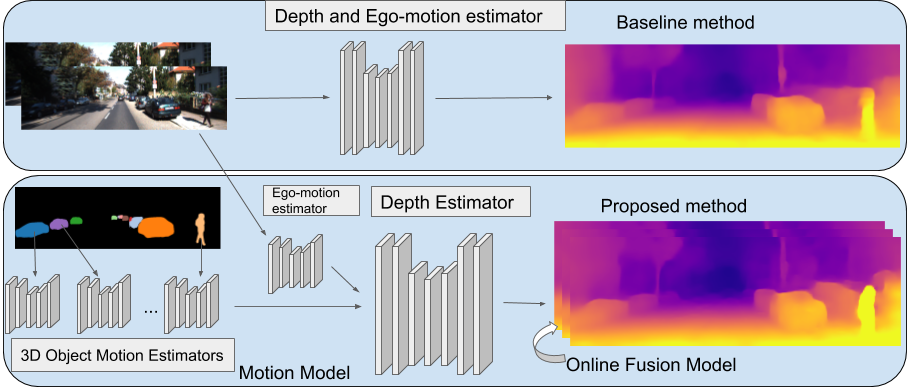
\includegraphics[width=\textwidth]{figs/aproach_depth.png}
  \end{center}
  \caption{struct2depthのアプローチ(https://sites.google.com/view/struct2depth)}
  \label{fig:approach_depth}
\end{figure}

\newpage
\section{物体検出システムについて}
%YOLOとかの話
物体検出を行うライブラリは様々あり,Fast R-CNNs\cite{ren2015faster},Mask R-CNN\cite{he2017mask},SSD\cite{liu2016ssd}といった手法が挙げられる.
それぞれCNNと呼ばれる畳み込みネットワークを利用し物体検出を行なっている点は同じだが,CNNの層や物体検出を行う際の手法がわずかながらに異なっている.
本研究では物体検出手法としてYOLO(You Only Look Once)\cite{yolov3}\figref{fig:yolo_system}\figref{fig:yolo_network}と呼ばれる物体検出手法を用いる.
YOLOは上記の3つの手法と比較して畳み込みネットワークやニューラルネットワークがシンプルな構造になっているにもかかわらず,高い検出率を誇っている.
また,構造が比較的シンプルなため演算処理にかかるスピードが速く,リアルタイムでの処理にも適している.
本研究では,YOLOがMicrosoft COCO datasetを機械学習したものを利用し,ドライブレコーダーに写っている自動車,トラック,バスを主に検出させ,距離推定及びその結果からシステムの評価を行う.

\begin{figure}[htbp]
  \begin{center}
    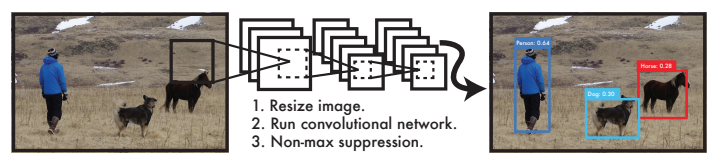
\includegraphics[width=\textwidth]{figs/Yolo_Detection_system.png}
    \caption{YOLOの物体検出システム\cite{yolov3}}
    \label{fig:yolo_system}
  \end{center}
\end{figure}

\begin{figure}[htbp]
  \begin{center}
    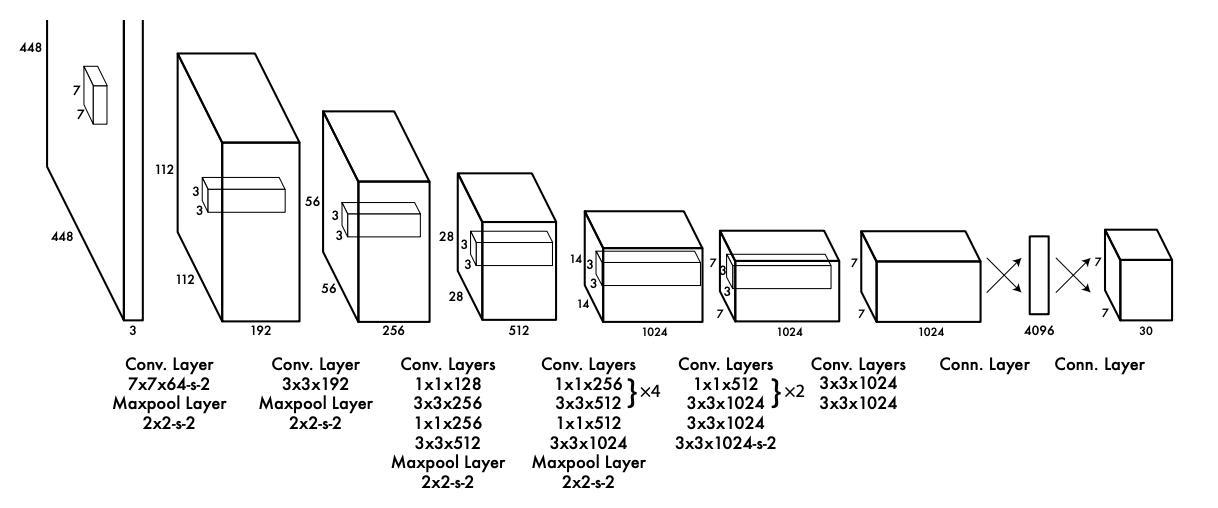
\includegraphics[width=\textwidth]{figs/yolo_architecture.png}
    \caption{YOLOのネットワーク構成図\cite{yolov3}}
    \label{fig:yolo_network}
  \end{center}
 \end{figure}
 
 \section{まとめ}
 本章では本研究における関連研究について述べた.
 次章では,問題に対する本研究のアプローチおよび本研究のシステムの設計と実装について述べる.